\documentclass{tufte-handout}

%\geometry{showframe}% for debugging purposes -- displays the margins

\usepackage{amsmath}

% Set up the images/graphics package
\usepackage{graphicx}
\setkeys{Gin}{width=\linewidth,totalheight=\textheight,keepaspectratio}
\graphicspath{{graphics/}}

\title{Mic Board: A Guide to Assembly}
\author[EE 16B]{EE 16B}
\date{30 January 2018}% if the \date{} command is left out, the current date will be used

% The following package makes prettier tables.  We're all about the bling!
\usepackage{booktabs}

% The units package provides nice, non-stacked fractions and better spacing
% for units.
\usepackage{units}

\usepackage{float}

% The fancyvrb package lets us customize the formatting of verbatim
% environments.  We use a slightly smaller font.
\usepackage{fancyvrb}
\fvset{fontsize=\normalsize}

% Small sections of multiple columns
\usepackage{multicol}

% Provides paragraphs of dummy text
\usepackage{lipsum}

% These commands are used to pretty-print LaTeX commands
\newcommand{\doccmd}[1]{\texttt{\textbackslash#1}}% command name -- adds backslash automatically
\newcommand{\docopt}[1]{\ensuremath{\langle}\textrm{\textit{#1}}\ensuremath{\rangle}}% optional command argument
\newcommand{\docarg}[1]{\textrm{\textit{#1}}}% (required) command argument
\newenvironment{docspec}{\begin{quote}\noindent}{\end{quote}}% command specification environment
\newcommand{\docenv}[1]{\textsf{#1}}% environment name
\newcommand{\docpkg}[1]{\texttt{#1}}% package name
\newcommand{\doccls}[1]{\texttt{#1}}% document class name
\newcommand{\docclsopt}[1]{\texttt{#1}}% document class option name

\begin{document}

\maketitle% this prints the handout title, author, and date
\linebreak\
\begin{abstract}
\noindent This week in lab, we will be assembling the mic board PCB (Printed Circuit Boards) that we will be using in the Color Organ Lab and for your final project, the robot car SIXT33N.
\end{abstract}
\begin{figure}
  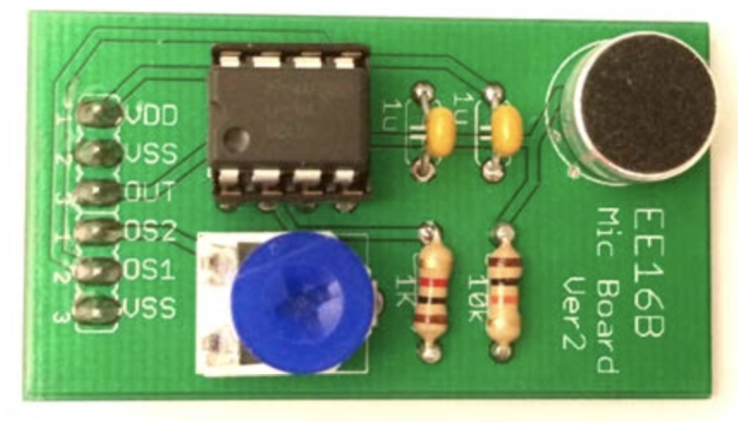
\includegraphics{miccomplete.png}
  \label{fig:textfig}
  \setfloatalignment{b}
\end{figure}
%\printclassoptions

\section{\underline{\textbf{Materials:}}}\label{sec:page-layout}


\begin{enumerate}
% \begin{marginfigure}[H]
% 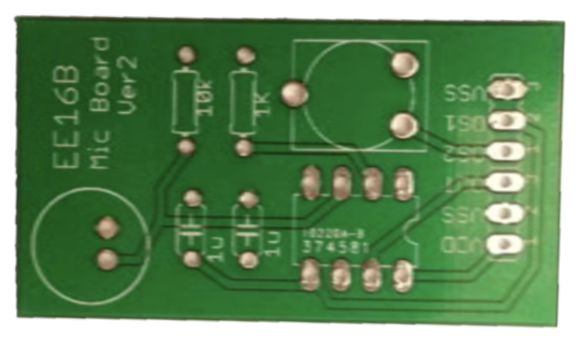
\includegraphics[width=\linewidth]{pcb.png}
%   \label{fig:marginfig}
% \end{marginfigure}
    \item 1 x microphone
    \item 1 x op amp
    \item 1 x 8-pin socket (not in kit, these will be handed out)
    \item 2 x 1 $\mu$F Capacitors (code 105 - not in kit, get these from cabinet)
\begin{marginfigure}
\centering
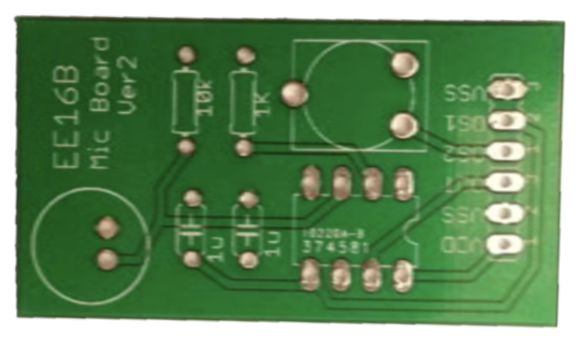
\includegraphics[width=\linewidth]{pcb.png}
\label{fig:marginfig}
\end{marginfigure}
    \item 1 x 10 k$\Omega$ Resistor
    \item 1 x 1 k$\Omega$ Resistor
    \item 1 x 50 k$\Omega$ Potentiometer
    \item 6 x Jumper pins (don't break apart!)
    \item 1 x MicBoard PCB
\end{enumerate}

\linebreak
\noindent All of the above materials (except for the PCB, capacitors, and IC socket) should be found in your parts kit. Check the resistors and capacitor values carefully! The two charts on the next page should be helpful. Note that all resistors we use have 4 colored bands, not 5.
\begin{figure*}[h!]
  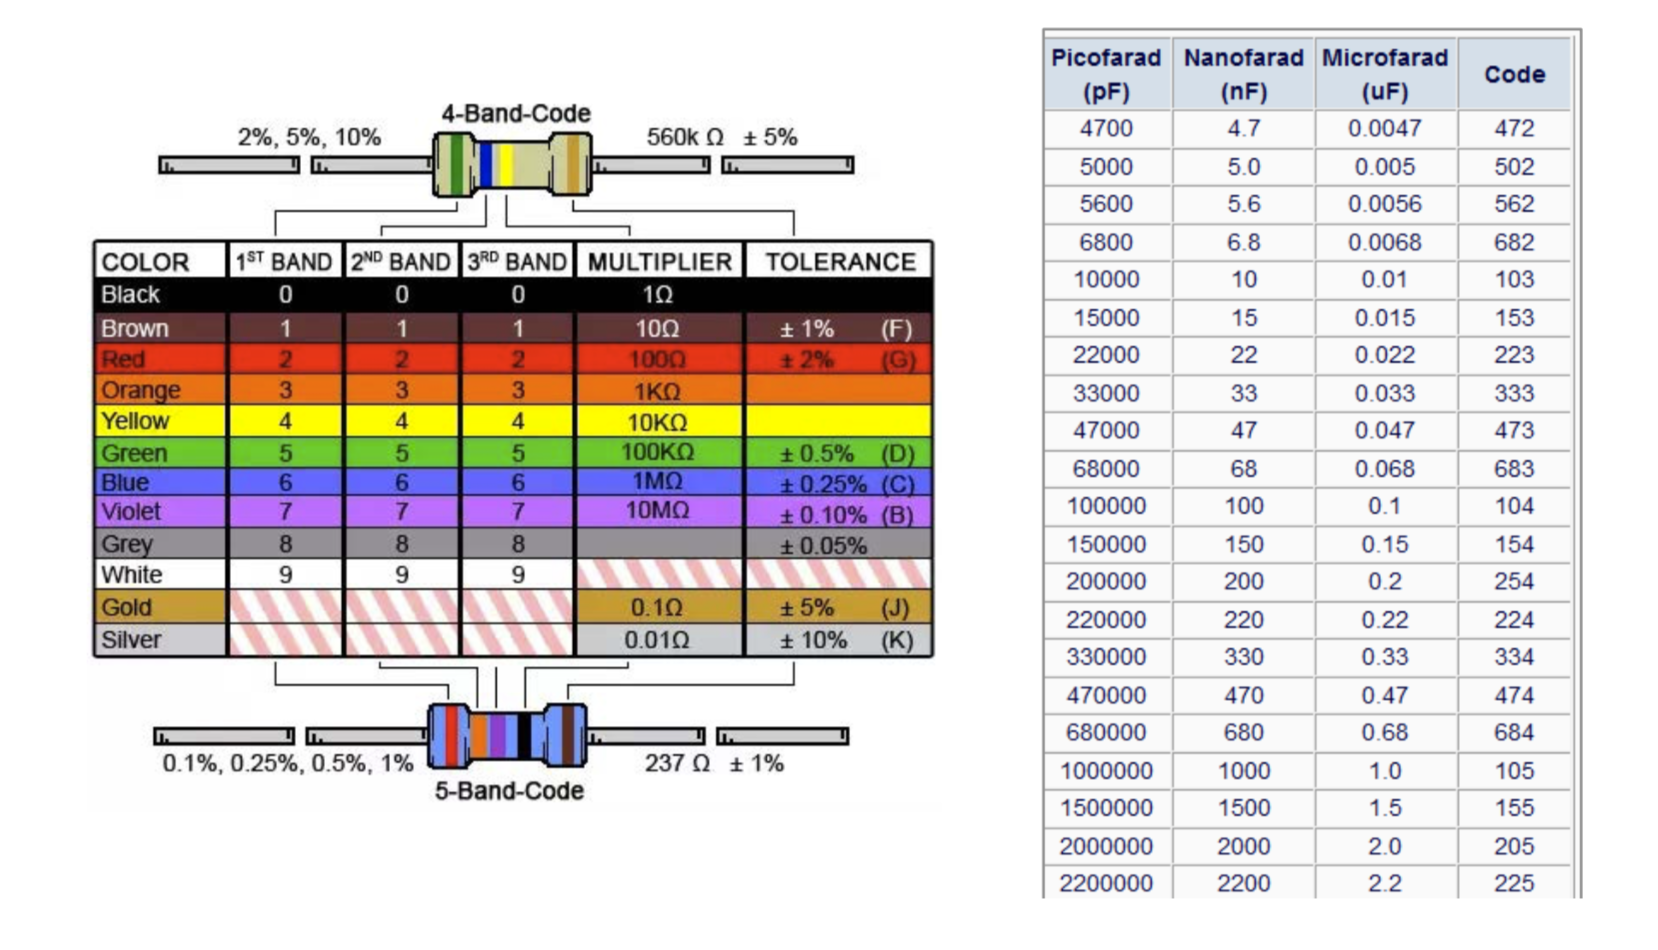
\includegraphics[width=\linewidth]{resistorchart.png}%
  \label{fig:fullfig}%
\end{figure*}

\clearpage

\section{\underline{\textbf{Assembly:}}}\label{sec:page-layout}
\noindent You can review how to solder parts here:\\ \url{https://www.youtube.com/watch?v=eU4t0Yko9Uk}

\medskip
\noindent Each lab station should have a soldering station with an iron and a sponge. Some notes:
\begin{itemize}
\item[--] Make sure the sponge is damp before wiping the hot iron; a squirt bottle can be found at the GSI desk
\item[--] TURN OFF the soldering station when not in use, and double check that it is off before leaving lab
\item[--] Make sure to solder in areas with proper ventilation (ie: don't breathe in the fumes!)
\item[--] Wash your hands before eating! (You should do this after lab anyway)
\end{itemize}

\bigskip
Each component is marked on the PCB. Make sure to put them in the right spots! A few things to be aware of:
\begin{itemize}
\item[--] The microphone is \textit{polarized}. This means that it matters which way we install it on the board. Make sure that the `ground side`\ is on the right (the mic should fit in the circle):
\begin{figure}
  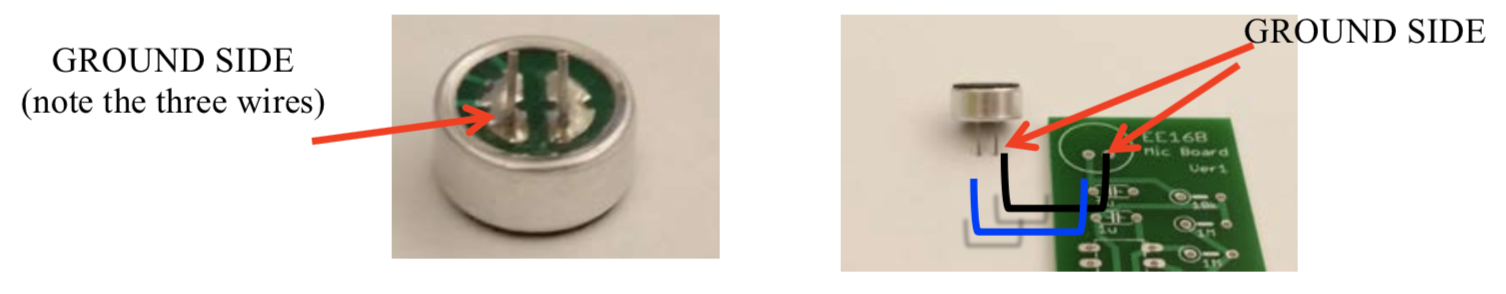
\includegraphics{groundside.png}
  \label{fig:textfig}
  \setfloatalignment{b}
\end{figure}
\item[--] Don`t solder the op-amp directly! Solder the socket to the board, that way we can swap out op-amps.
\item[--] Keep all 6 jumper pins connected. This will make it a lot easier to solder them in.
\item[--] Make sure the \textbf{long side} (of the jumpers) is pointing \textit{down}. This means that you will insert the jumpers \textbf{from below} and solder  \textbf{on the top side} of the board (we will use these to plug the mic board into our breadboards)

\begin{figure*}[h!]
  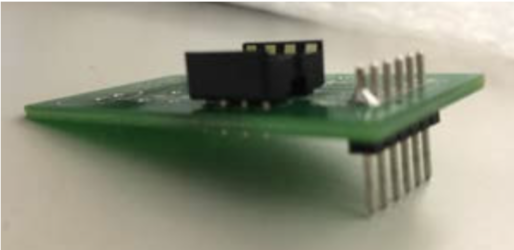
\includegraphics{sideview.png}
  \label{fig:textfig}
%   \setfloatalignment{b}
\end{figure*}

\item[--] The color/shape of the capacitors does \textbf{not} matter - only the numeric code marked on them. You will be using two 1 $\mu$F capacitors, which are coded \textbf{105}.
\item[--] Note which way the op-amp needs to be placed in the socket. Pin one should be in the \textbf{lower right hand corner!} You can tell which way the op amp needs to be by looking at the white outline on the board. The little notch on the bottom tells us that this is where the ``top`` of the op amp should be

\begin{figure*}[h!]
  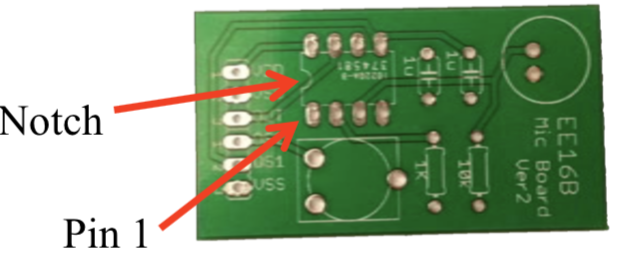
\includegraphics[]{notchpin.png}\centering\nonumber
  \label{fig:textfig}
  \setfloatalignment{b}
\end{figure*}

\item[--] Make sure you use enough solder to make a solid connection. There should be a little blob that`s big enough to cover the entire metal contact on the board. If you aren`t sure, ask your GSI.
\end{itemize}
\newpage
\section{\underline{\textbf{Operation:}}}\label{sec:page-layout}
\noindent The Mic Boards use the schematic below:

\begin{figure*}[h!]
  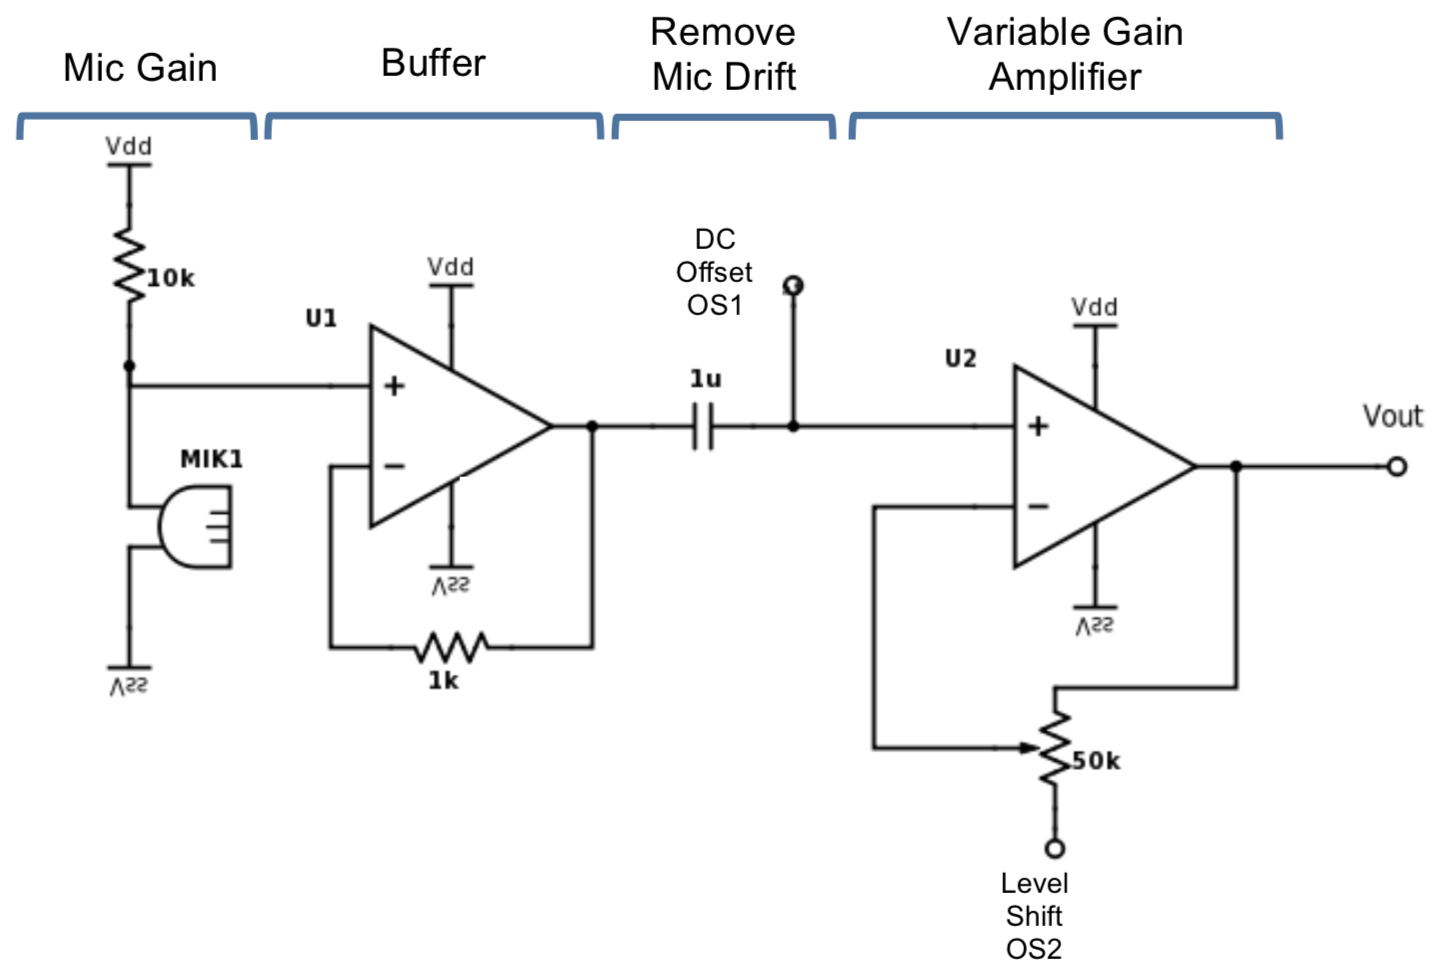
\includegraphics[width=\linewidth]{schematic.png}%
  \label{fig:fullfig}%
\end{figure*}

\medskip
\noindent \newline You might have also noticed that there is another 1 $\mu$F capacitor on your mic board. This is known as a ``decoupling capacitor`` and is used to help filter out noise that might be present in the power rails. It is connected directly between VDD and VSS.
\medskip
\noindent \newline Don`t worry too much about what each of the stages do right now, we will be looking into them in more depth in a couple of weeks.
\medskip
\noindent \newline The microphone can be thought of as a variable current source; it produces current in reaction to sound input. Since we want to work with voltages, we put the mic in series with the 10 k$\Omega$ resistor, then pick off the voltage drop across the resistor.
\medskip
\noindent \newline The next stage is a buffer to keep the rest of the circuit from influencing our mic signal. After that, the 1 $\mu$F capacitor is used to remove the DC offset from the microphone signal (we will discuss this more during the project). This is essentially a high-pass filter.
\medskip
\noindent \newline The last stage is a variable non-inverting amplifier. The 50 k$\Omega$ potentiometer can be used to tune the gain to whatever is needed. We will talk more about what the DC offset and Level Shift terminals mean when we start the project, but for now we will connect them to ground.
\newpage

\section{\underline{\textbf{Testing:}}}\label{sec:page-layout}

\noindent To test that your mic board is functioning properly, we will hook it up the oscilloscope. We will need to use four of the six pins we soldered in.

\linebreak\
\linebreak\
\noindent
VDD: Set this at 5 V
\par\noindent
VSS: Set this at -5 V (Only one must be connected)
\par\noindent
OUT: OScope probe point
\par\noindent
OS2: Set this to GND
\par\noindent
OS1: 100 k$\Omega$ resistor to ground

\begin{marginfigure}%
  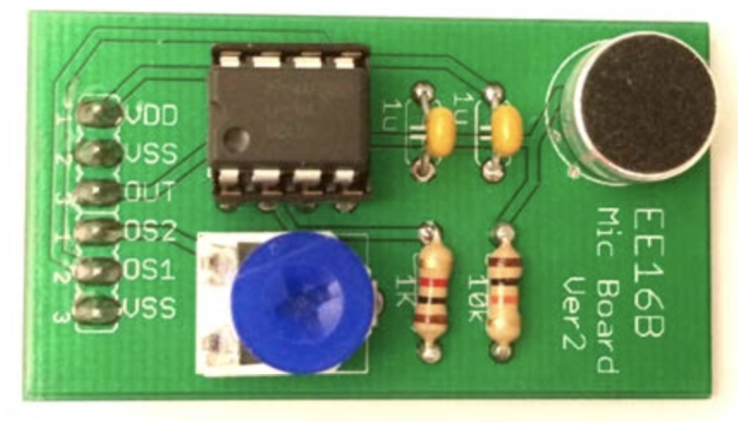
\includegraphics[width=\linewidth]{miccomplete.png}
  \label{fig:marginfig}
\end{marginfigure}

\bigskip
\newline
\noindent
\medskip
Note: set the time step to 10 ms/division!\par
\noindent
\medskip
Probe at the OUT terminal of the mic board, and try speaking into the microphone. You may not see anything at first. That's ok! The potentiometer sets the gain of our board. If the gain is too low, we won't see a signal, and if the gain is too high, it might rail.\par
\noindent
\medskip
Turn the potentiometer counter-clockwise for more gain and clockwise for less. There are screwdrivers at the TA desk. When adjusted appropriately, you should see a signal that responds when you make noise, centered around ground.

\end{document}
